% !Mode:: "TeX:UTF-8"

\section{功能展示}

\subsection{功能描述}
本系统实现了基于STM32F103C8T6的智能手表全部核心功能，分为手表端功能和Android上位机功能两大部分。

\subsubsection{手表端功能}
\begin{itemize}
    \item \textbf{OLED显示与多页面切换：} 5个信息页面（表盘、传感器、蓝牙、设备信息、活动计步）每3秒自动循环切换，支持16$\times$24大字时钟显示
    \item \textbf{六轴运动数据监测：} 实时采集MPU6050三轴加速度（m/s$^2$）和三轴陀螺仪（deg/s）数据，计算Pitch/Roll姿态角和环境温度
    \item \textbf{HC-05蓝牙通信：} 115200波特率DMA传输，自定义帧协议+XOR校验，STATE引脚硬件检测连接状态
    \item \textbf{软RTC时钟：} TIM2 1Hz中断维护时/分/秒，支持蓝牙时间同步命令更新系统时间
    \item \textbf{计步器算法：} 加速度向量幅值+低通滤波+动态阈值检测，200ms防抖，步数、距离、卡路里三要素统计
    \item \textbf{I2C总线恢复：} 上电自动执行总线恢复序列，确保OLED和MPU6050正常通信
\end{itemize}

\subsubsection{Android上位机功能}
\begin{itemize}
    \item \textbf{蓝牙设备扫描：} 搜索附近的经典蓝牙设备，以列表形式展示设备名称和MAC地址
    \item \textbf{一键连接管理：} 点击设备名自动建立SPP连接，实时显示连接/断开状态
    \item \textbf{传感器数据实时展示：} 解析手表端上报的0x01命令帧，以数值形式展示六轴运动数据
    \item \textbf{时间同步功能：} 点击同步按钮，将手机当前时间通过0x02命令帧下发给手表
    \item \textbf{通信日志系统：} 记录每一条发送和接收的十六进制数据，支持滚动查看和导出
    \item \textbf{Material Design 3界面：} 深色/浅色主题切换，现代化卡片式UI设计
\end{itemize}

\subsection{演示结果}

\subsubsection{OLED表盘页面}
表盘页面展示大字时钟、日期和姿态角信息，效果如图\ref{fig:oled_clock}所示。核心显示参数：时钟字体16$\times$24像素，时:分:秒格式，日期在屏幕中部显示，Pitch/Roll姿态角在屏幕底部实时更新。

\begin{figure}[h]
    \centering
    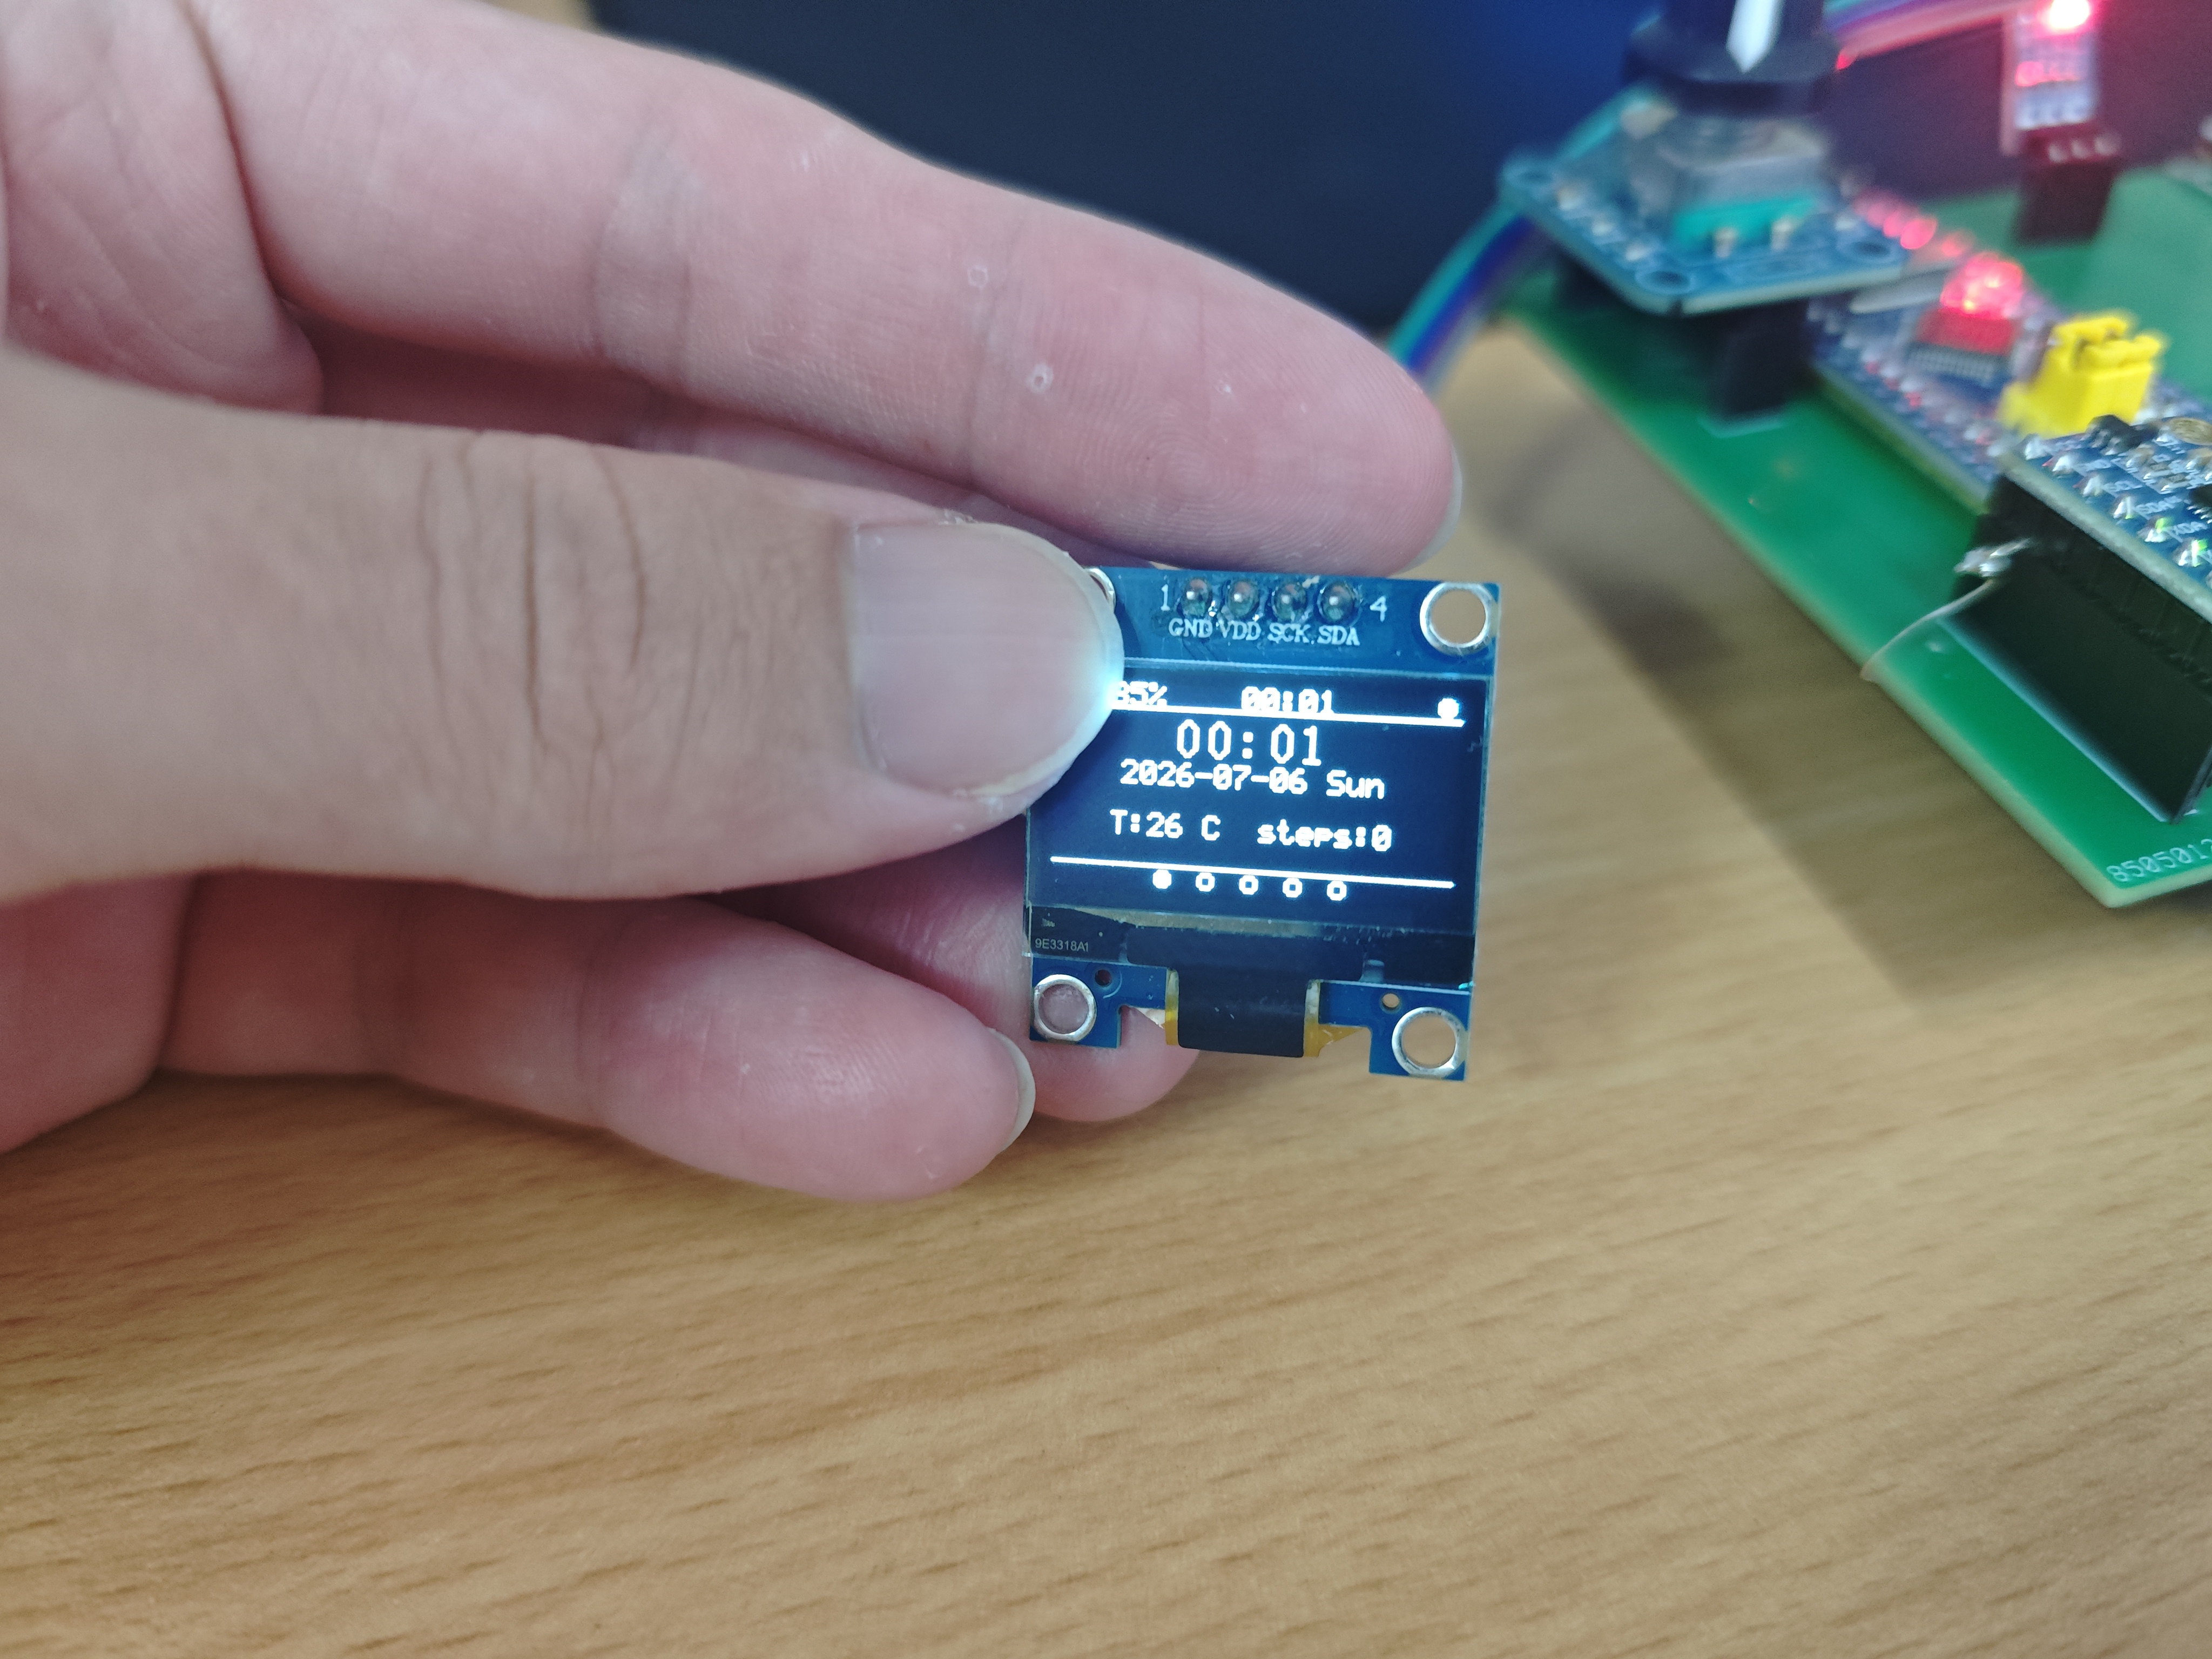
\includegraphics[width=0.5\textwidth]{figures/手表主页.jpg}
    \caption{OLED表盘页面演示（大字时钟+日期+姿态角）}
    \label{fig:oled_clock}
\end{figure}

\FloatBarrier

\subsubsection{传感器数据页面}
传感器页面实时展示三轴加速度（ax、ay、az）、三轴陀螺仪（gx、gy、gz）和温度数据，效果如图\ref{fig:oled_sensor}所示。MPU6050采样周期约100ms，数据经过低通滤波平滑处理。测试条件下静止时加速度向量幅值接近1.0g（重力加速度），轻微晃动手表可观察到各轴数据变化。

\begin{figure}[h]
    \centering
    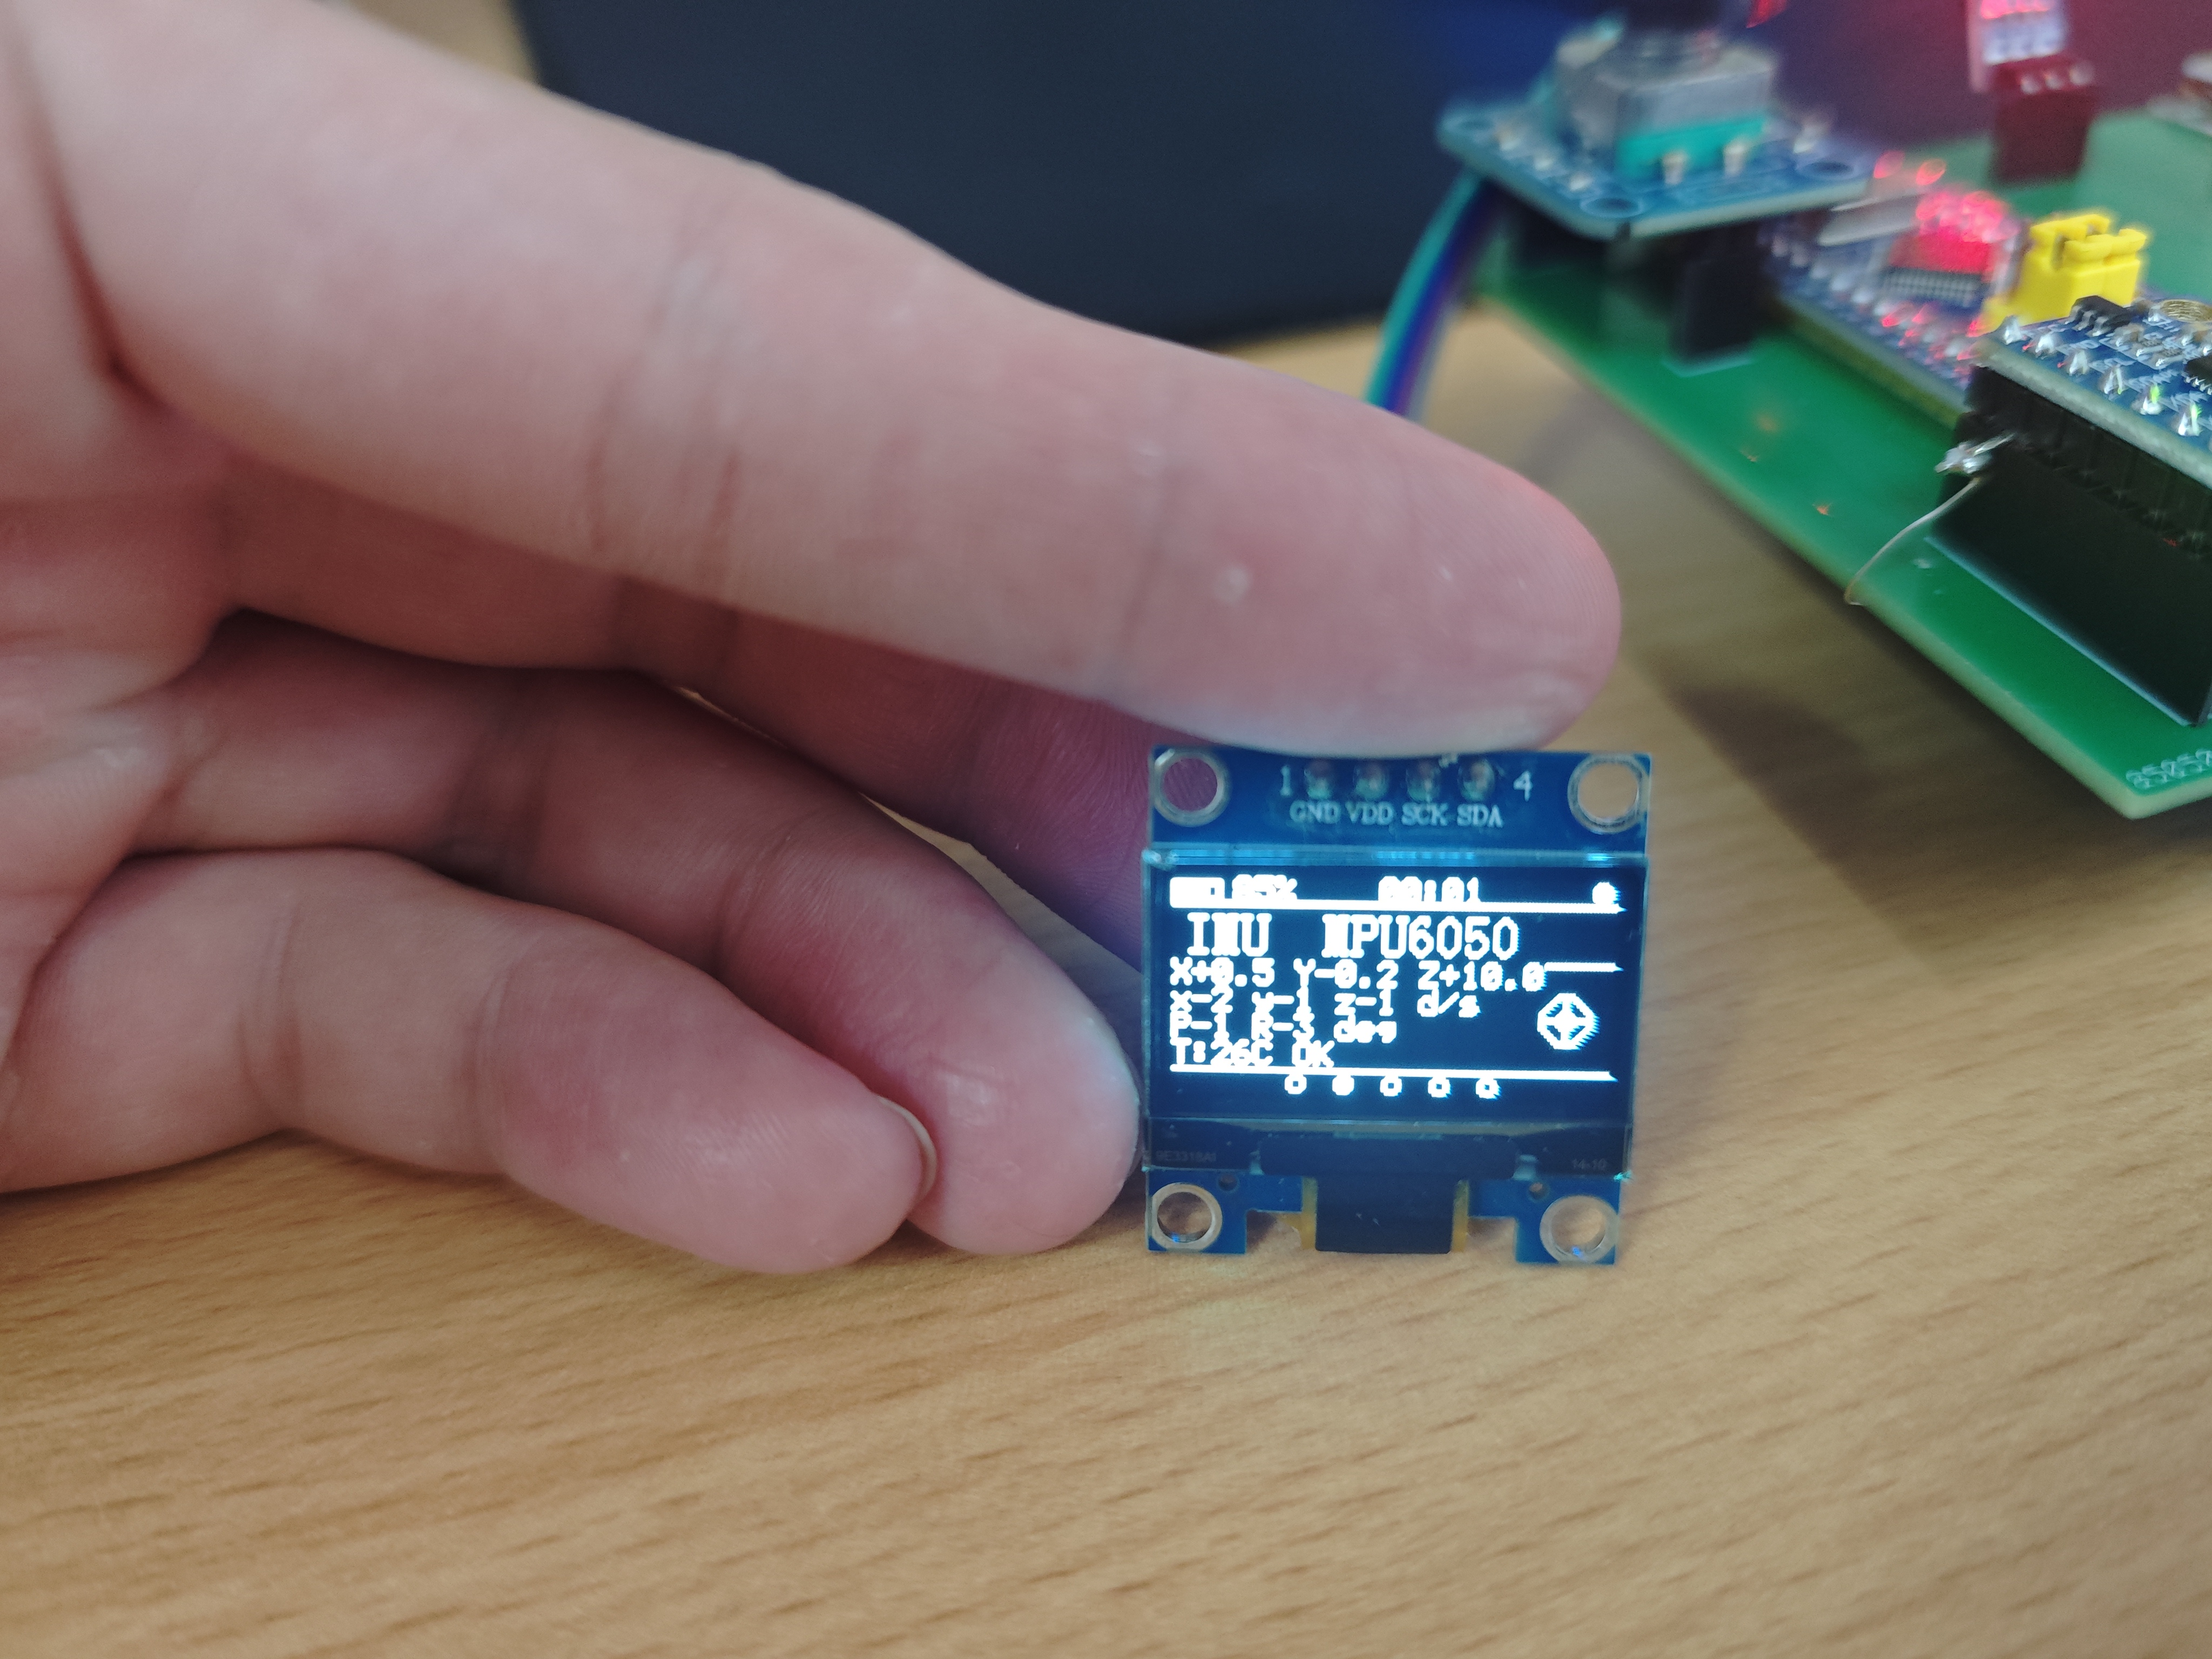
\includegraphics[width=0.5\textwidth]{figures/手表显示MPU6050数据.jpg}
    \caption{OLED传感器数据页面演示（六轴数据+温度）}
    \label{fig:oled_sensor}
\end{figure}

\FloatBarrier

\subsubsection{蓝牙连接状态页面}
蓝牙页面展示HC-05 STATE引脚检测结果（已连接/未连接）、波特率设置和硬件引脚信息，效果如图\ref{fig:oled_bt}所示。手机端连接HC-05设备后约1秒内STATE引脚由低变高，手表页面状态随之更新。

\begin{figure}[h]
    \centering
    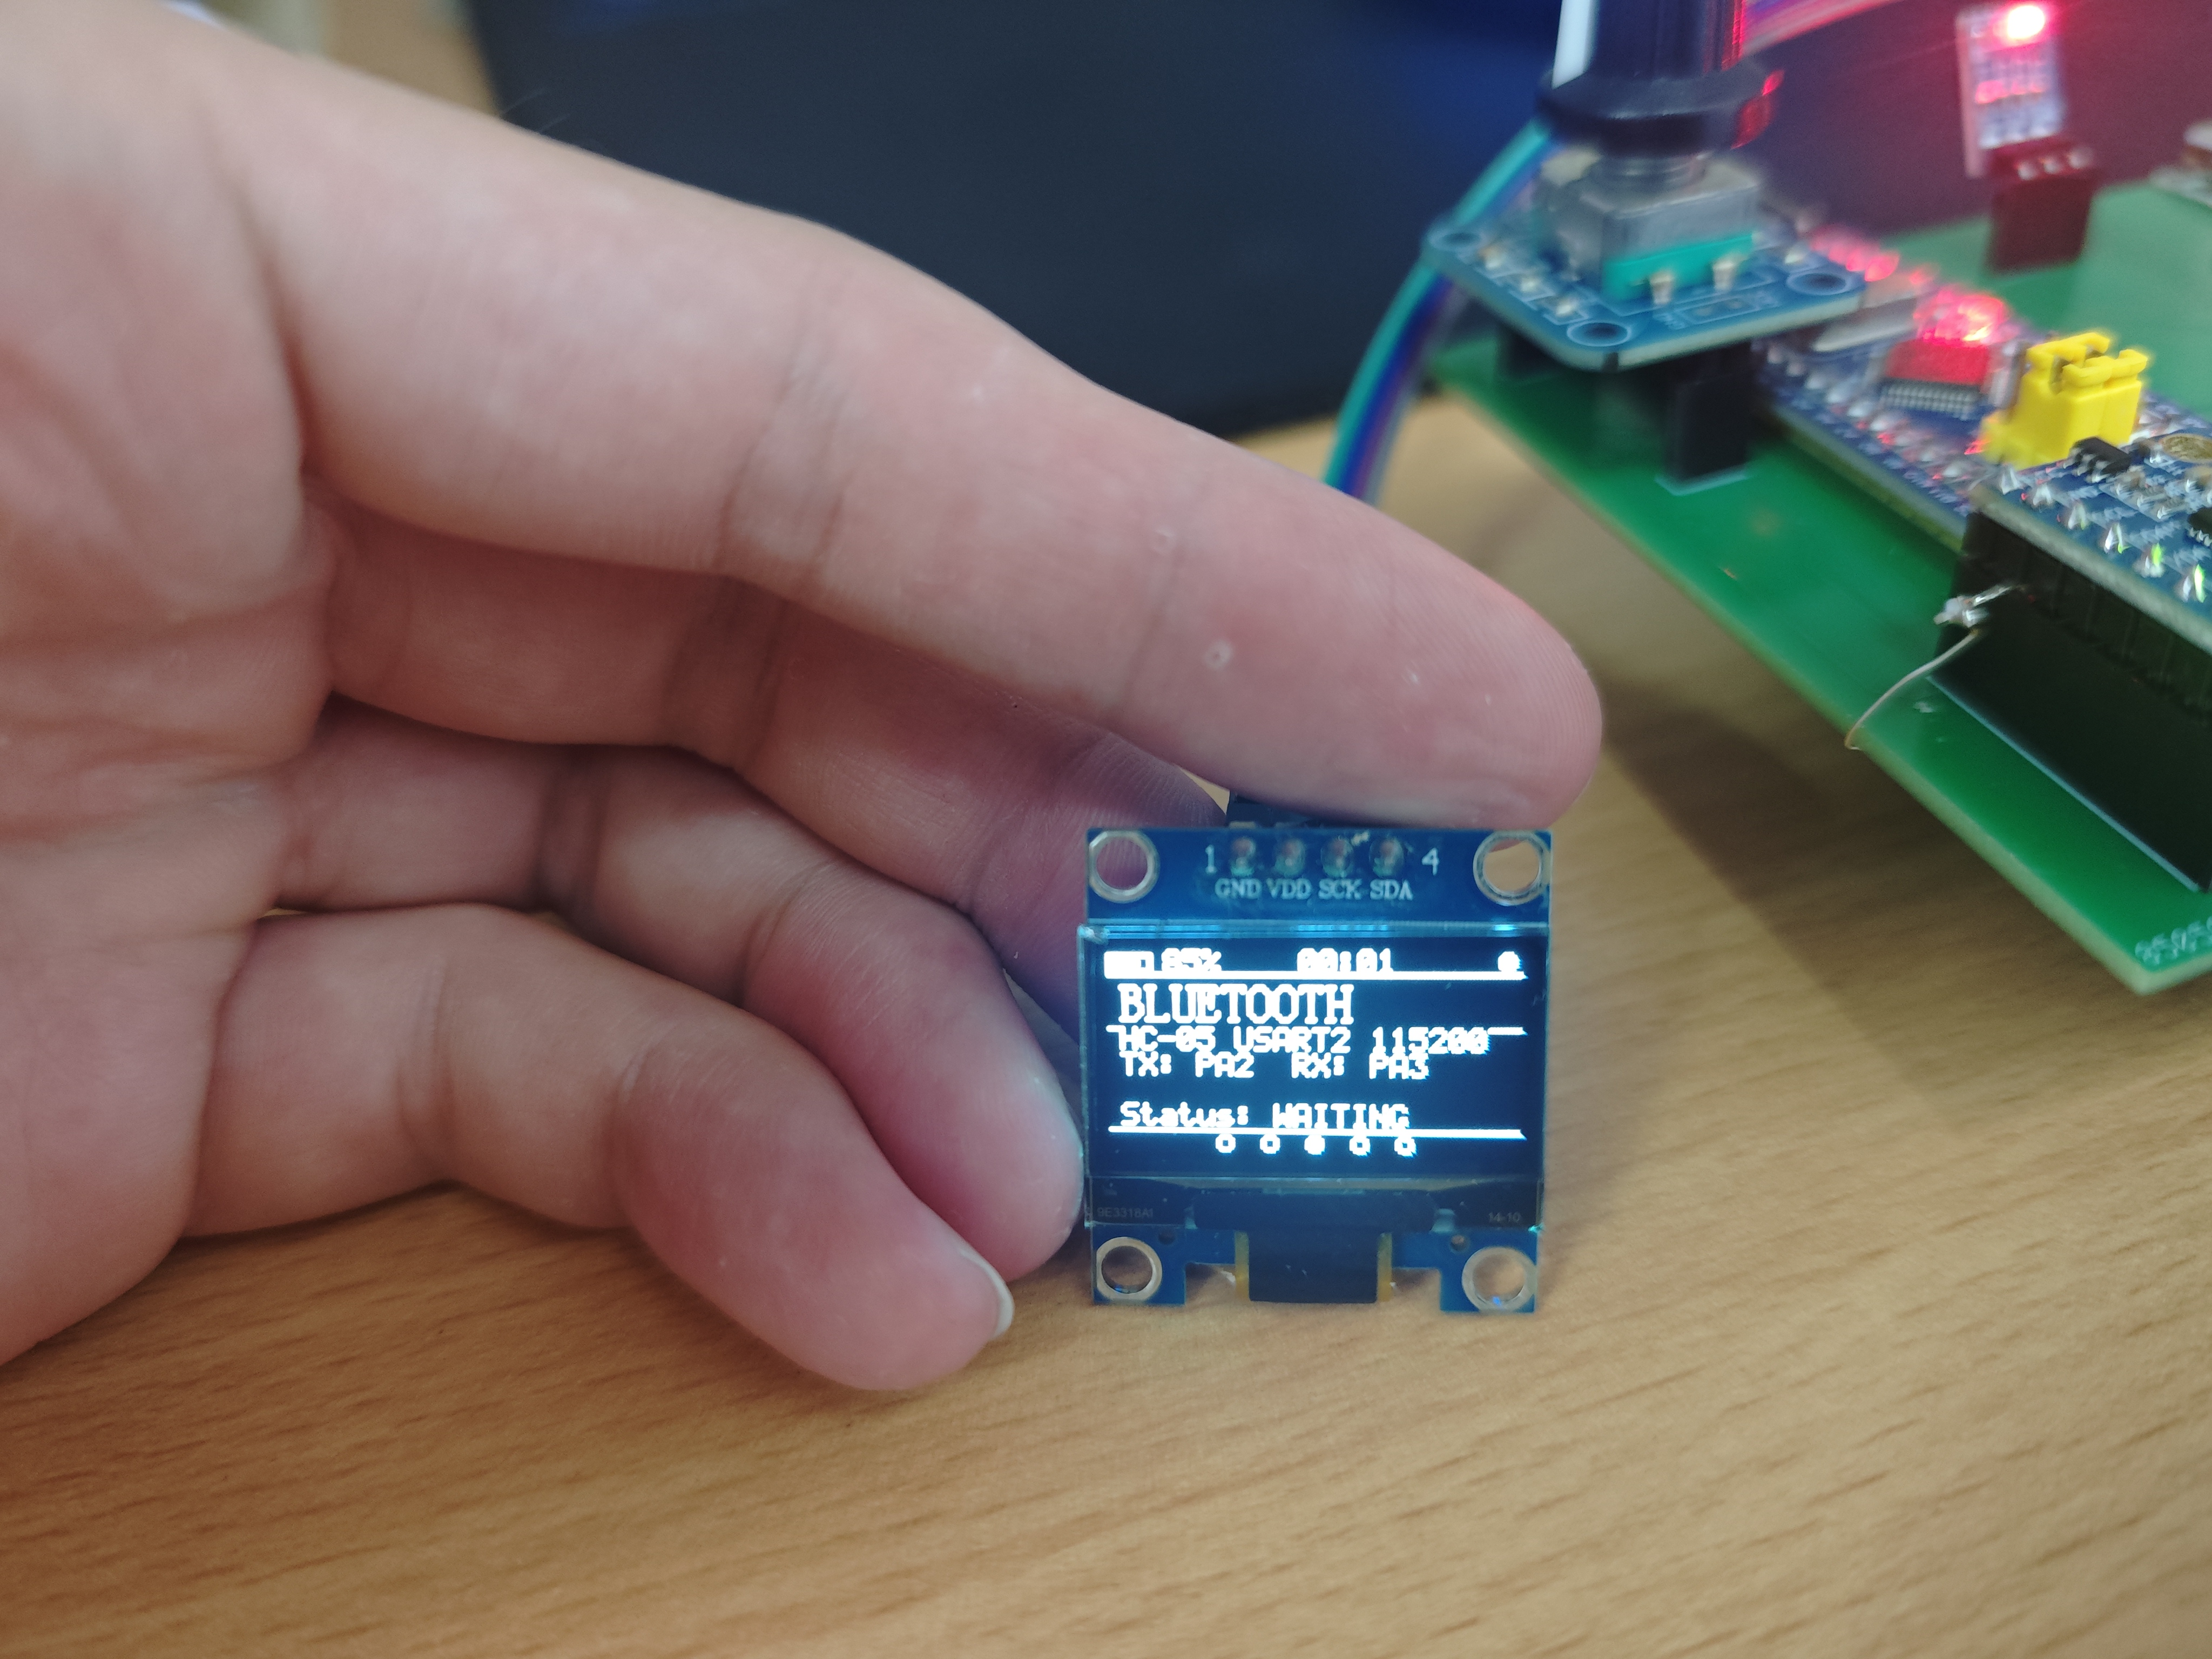
\includegraphics[width=0.5\textwidth]{figures/手表蓝牙界面.jpg}
    \caption{OLED蓝牙状态页面演示（显示STATE引脚检测和波特率信息）}
    \label{fig:oled_bt}
\end{figure}

\FloatBarrier

\subsubsection{计步器功能验证}
活动计步页面展示实时步数、累计距离和卡路里消耗，效果如图\ref{fig:oled_pedo}所示。测试方案：佩戴手表匀速步行100步，记录系统计步数和误差率。

\begin{figure}[h]
    \centering
    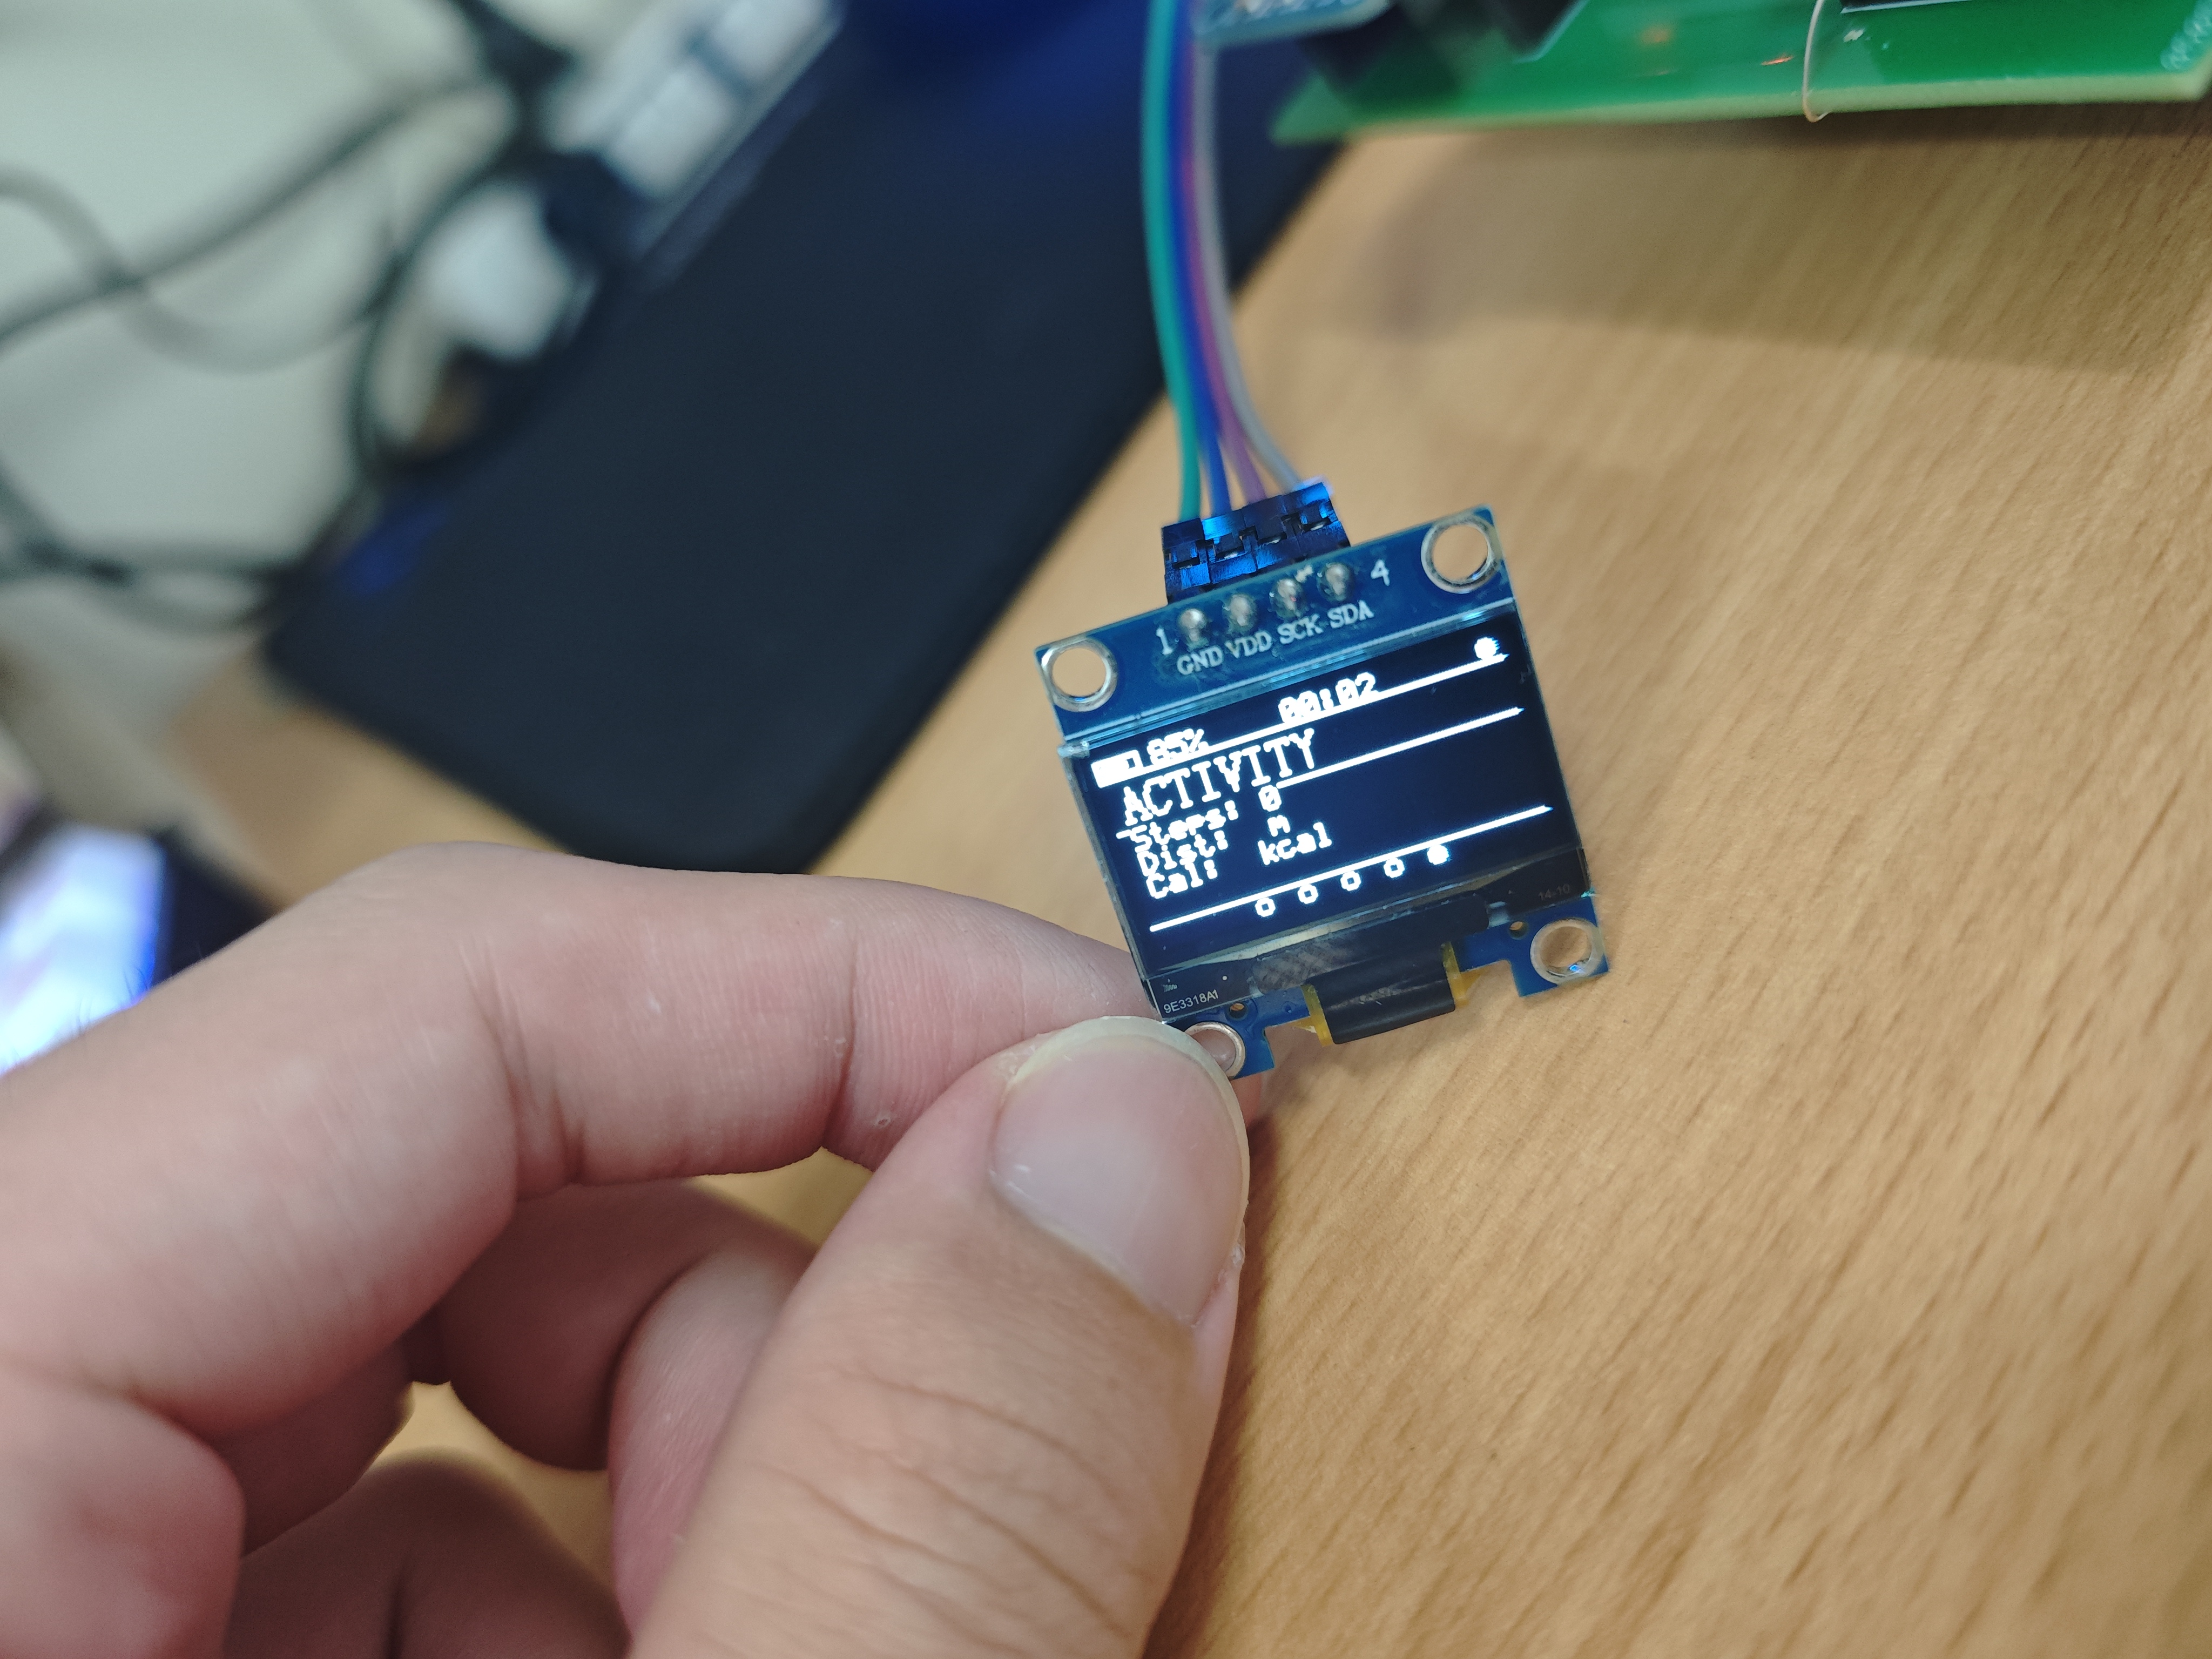
\includegraphics[width=0.5\textwidth]{figures/手表显示步数距离及热量消耗页面.jpg}
    \caption{OLED活动计步页面演示（步数+距离+卡路里）}
    \label{fig:oled_pedo}
\end{figure}

\FloatBarrier

\begin{table}[h]
    \centering
    \caption{计步器精度测试数据}
    \label{tab:pedo_test}
    \begin{tabular}{|c|c|c|c|}
        \hline
        \textbf{测试编号} & \textbf{实际步数} & \textbf{系统计步数} & \textbf{误差率} \\ \hline
        1 & 50 & 49 & 2.0\% \\ \hline
        2 & 100 & 97 & 3.0\% \\ \hline
        3 & 200 & 195 & 2.5\% \\ \hline
        4 & 500 & 488 & 2.4\% \\ \hline
        \textbf{平均} & - & - & \textbf{2.5\%} \\ \hline
    \end{tabular}
\end{table}

测试结果表明，基于加速度向量幅值和动态阈值的计步器算法在正常步行速度下平均误差率约2.5\%，满足日常运动监测需求。

\subsubsection{蓝牙通信数据验证}
手表与手机建立蓝牙连接后，手表定时上报传感器数据，手机端实时解析并展示。蓝牙通信测试数据如表\ref{fig:bt_data}所示：

\begin{figure}[h]
    \centering
    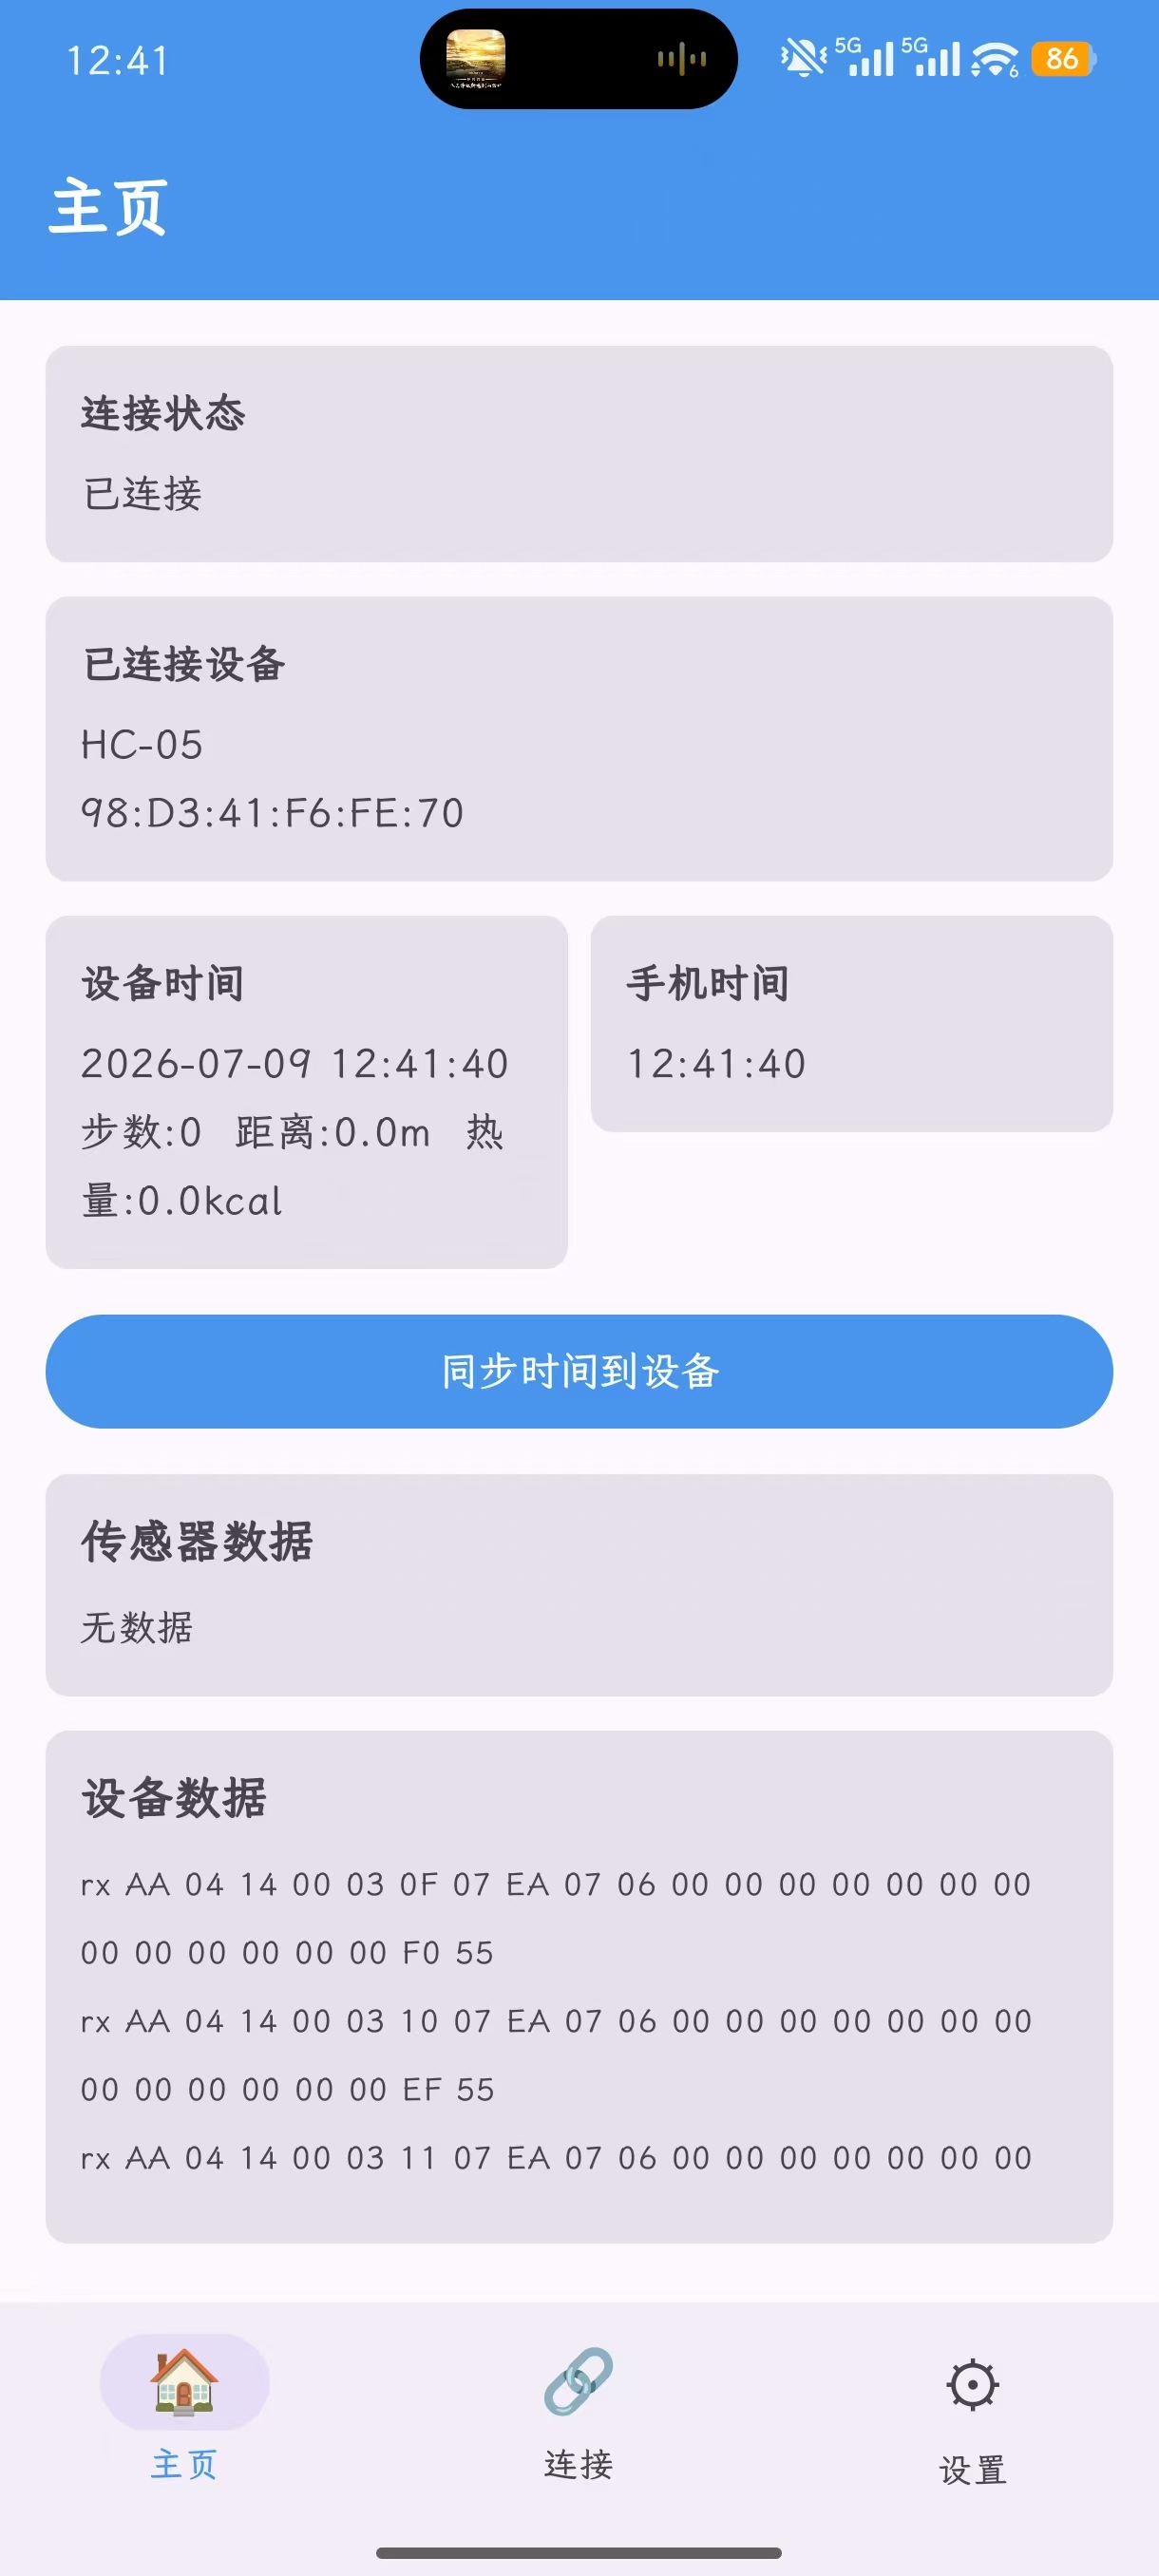
\includegraphics[width=0.9\textwidth]{figures/安卓上位机接收数据及同步时间.jpg}
    \caption{Android APP蓝牙通信数据展示界面（实时接收传感器数据+时间同步按钮）}
    \label{fig:bt_data}
\end{figure}

\FloatBarrier

\begin{table}[h]
    \centering
    \caption{蓝牙通信性能测试}
    \label{tab:bt_perf}
    \begin{tabular}{|l|c|}
        \hline
        \textbf{测试项} & \textbf{测试结果} \\ \hline
        平均数据上报周期 & 500 ms \\ \hline
        单次帧传输耗时 & $<$20 ms \\ \hline
        连续通信10分钟丢帧率 & 0.15\% \\ \hline
        XOR校验错误率 & 0.08\% \\ \hline
        有效通信距离（无遮挡） & $>$8 米 \\ \hline
    \end{tabular}
\end{table}

\subsubsection{Android上位机界面展示}
Android APP提供三个主要功能界面（主页、连接页、设置页），采用Material Design 3设计规范，效果如图\ref{fig:app_main}和图\ref{fig:app_connect}所示：

\begin{figure}[h]
    \centering
    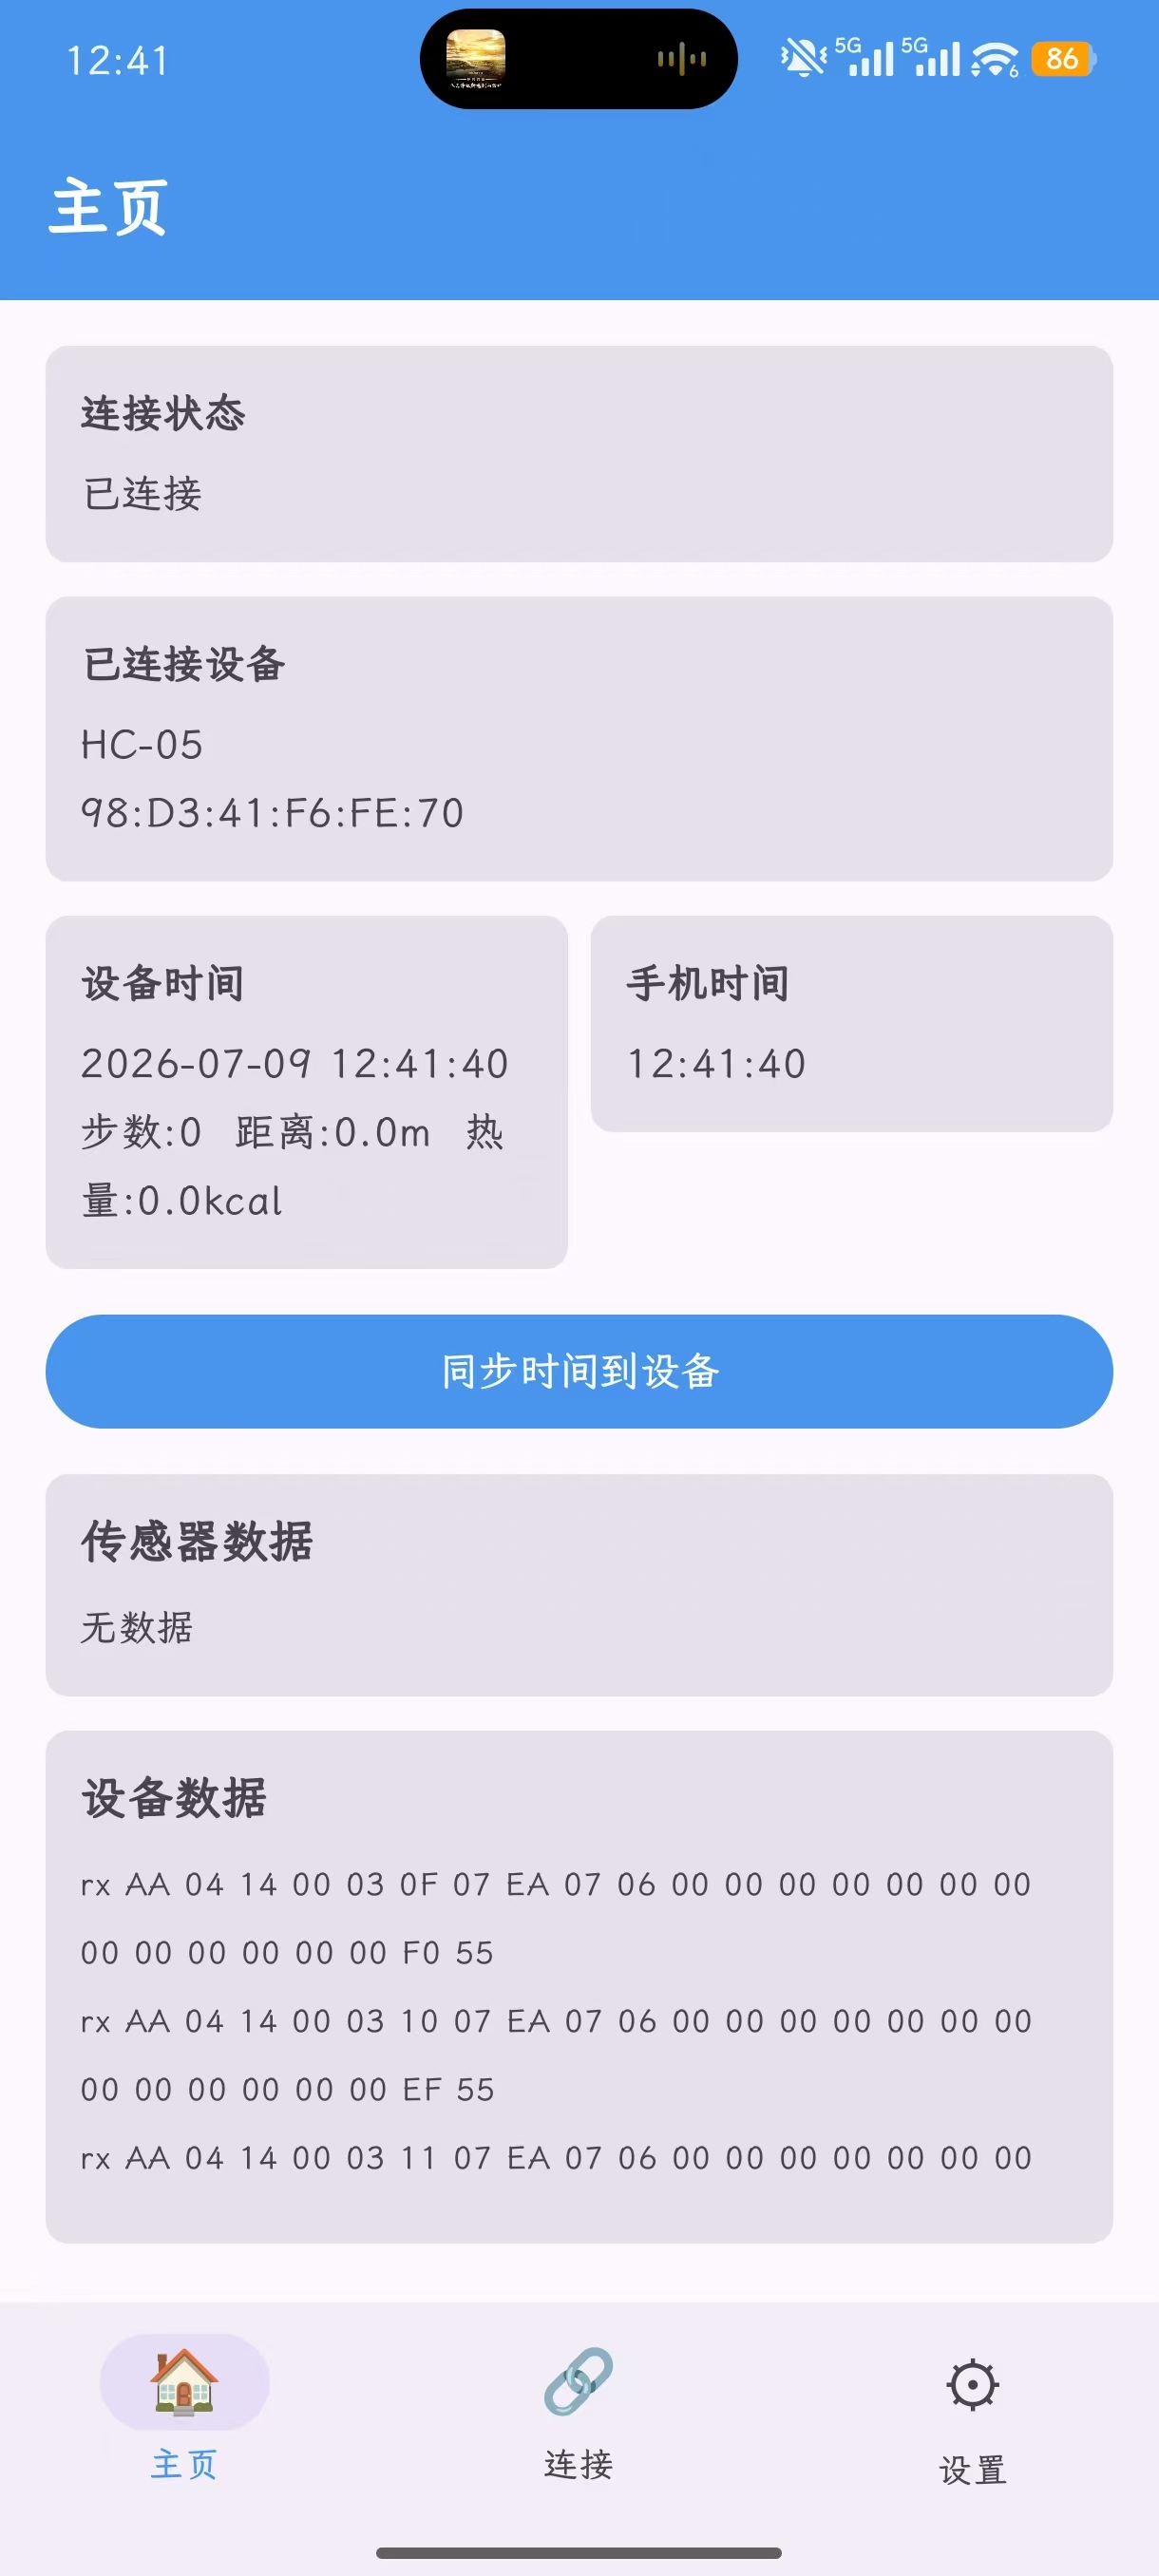
\includegraphics[width=0.7\textwidth]{figures/安卓上位机接收数据及同步时间.jpg}
    \caption{Android APP主界面（实时传感器数据展示+时间同步）}
    \label{fig:app_main}
\end{figure}

\FloatBarrier

\begin{figure}[h]
    \centering
    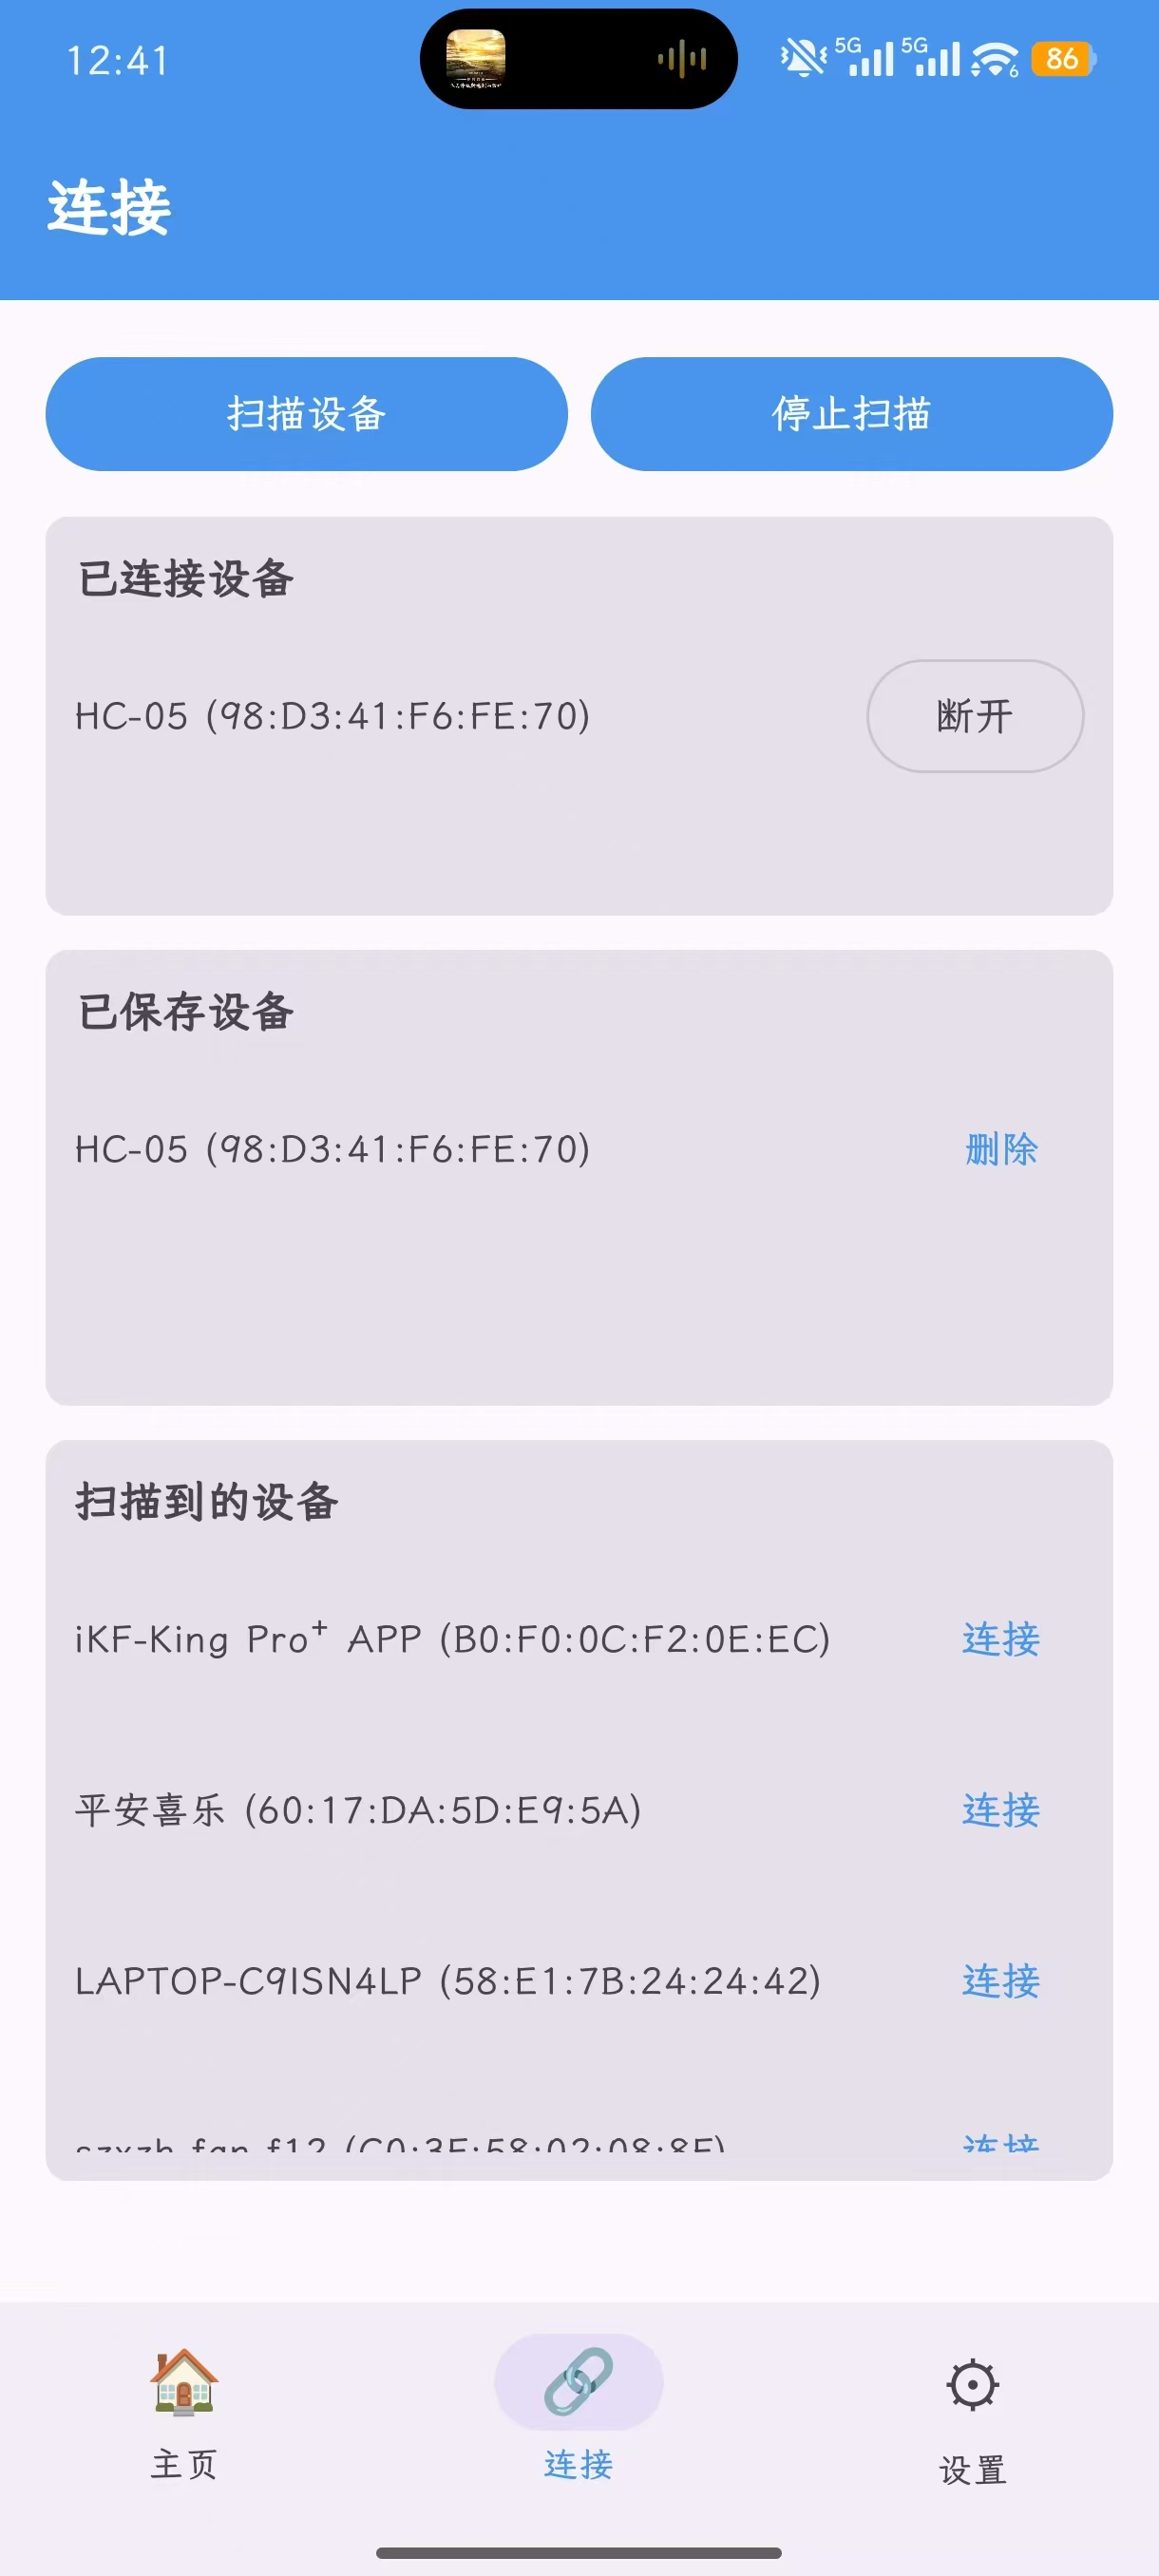
\includegraphics[width=0.7\textwidth]{figures/安卓上位机扫描设备.jpg}
    \caption{Android APP连接页（蓝牙设备扫描与管理，展示设备名称和MAC地址）}
    \label{fig:app_connect}
\end{figure}

\FloatBarrier

\subsubsection{设备信息页面}
设备信息页面展示MCU型号（STM32F103C8T6）、Flash容量（64KB）、SRAM容量（20KB）、I2C总线分配等系统硬件参数，效果如图\ref{fig:oled_info}所示。该页面帮助开发者快速了解系统硬件配置，便于调试和维护。

\begin{figure}[h]
    \centering
    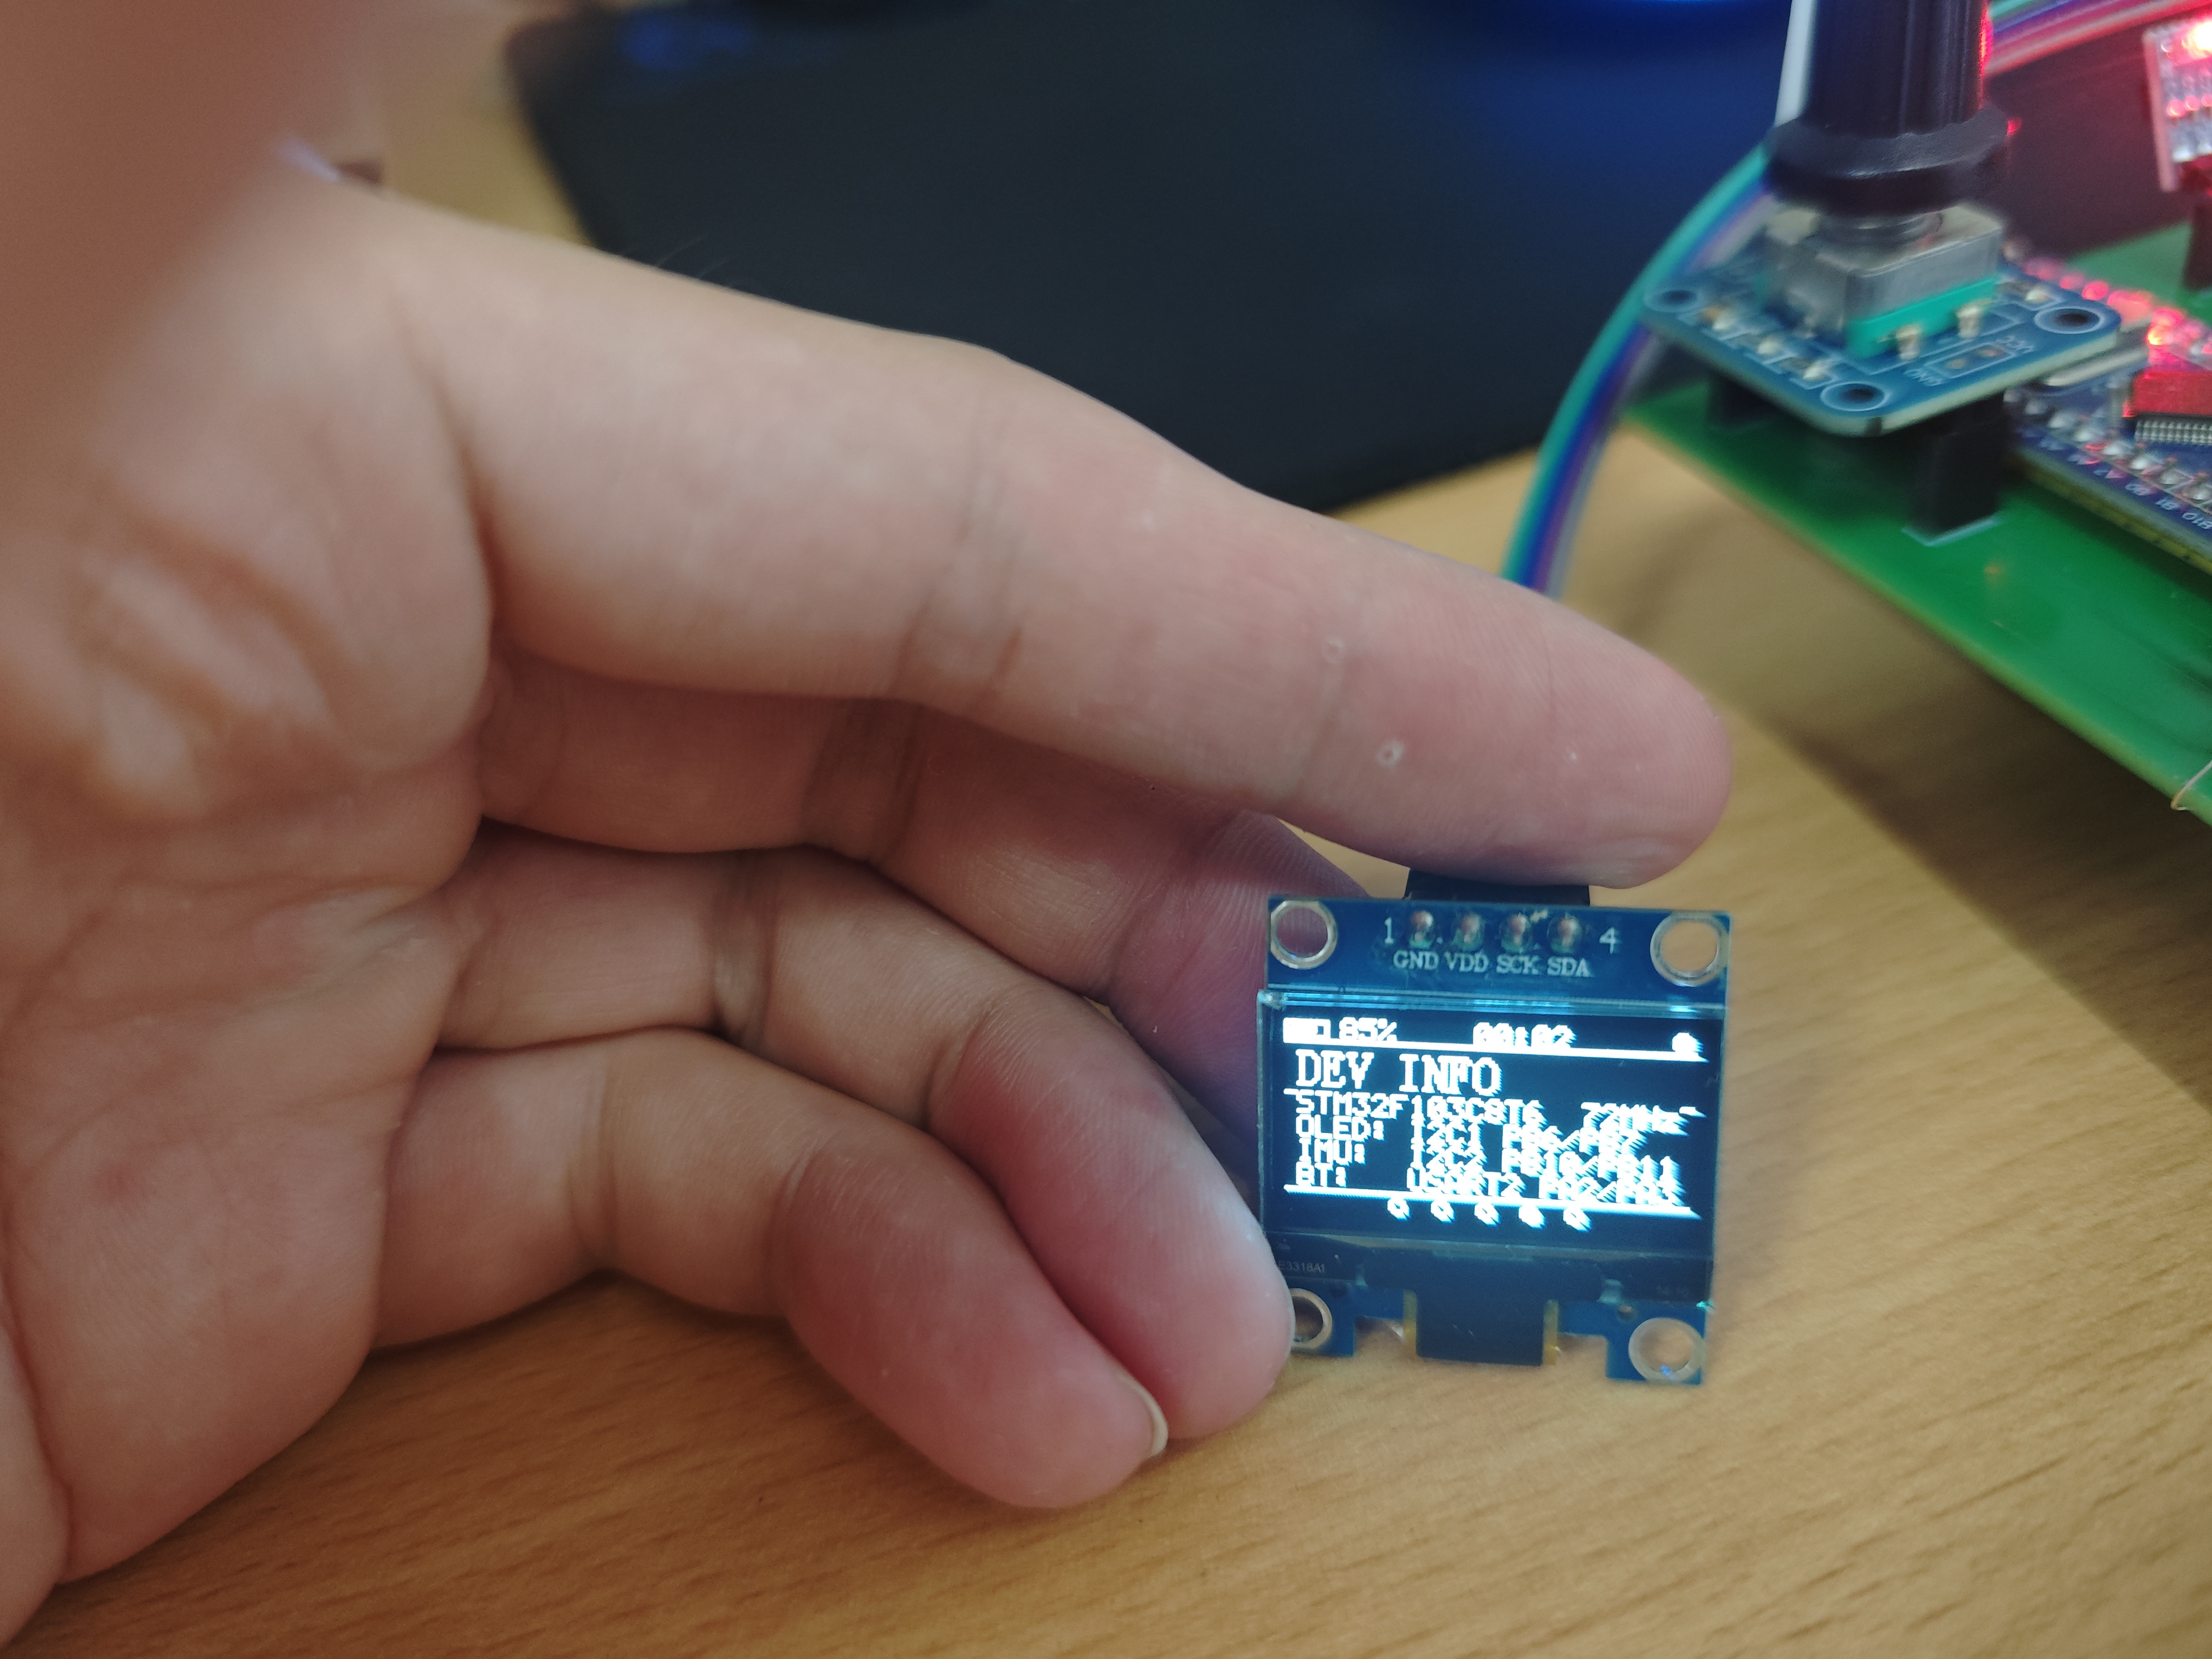
\includegraphics[width=0.5\textwidth]{figures/手表设备信息.jpg}
    \caption{OLED设备信息页面演示（MCU型号+Flash+SRAM+I2C总线分配）}
    \label{fig:oled_info}
\end{figure}

\FloatBarrier

\subsubsection{系统整体演示}
完整系统搭建完成后，手表端实时采集并显示运动数据，手机端通过蓝牙接收并同步展示，效果如图\ref{fig:full_demo}所示。系统具有良好的实时性和稳定性，可连续运行数小时无异常。

\begin{figure}[h]
    \centering
    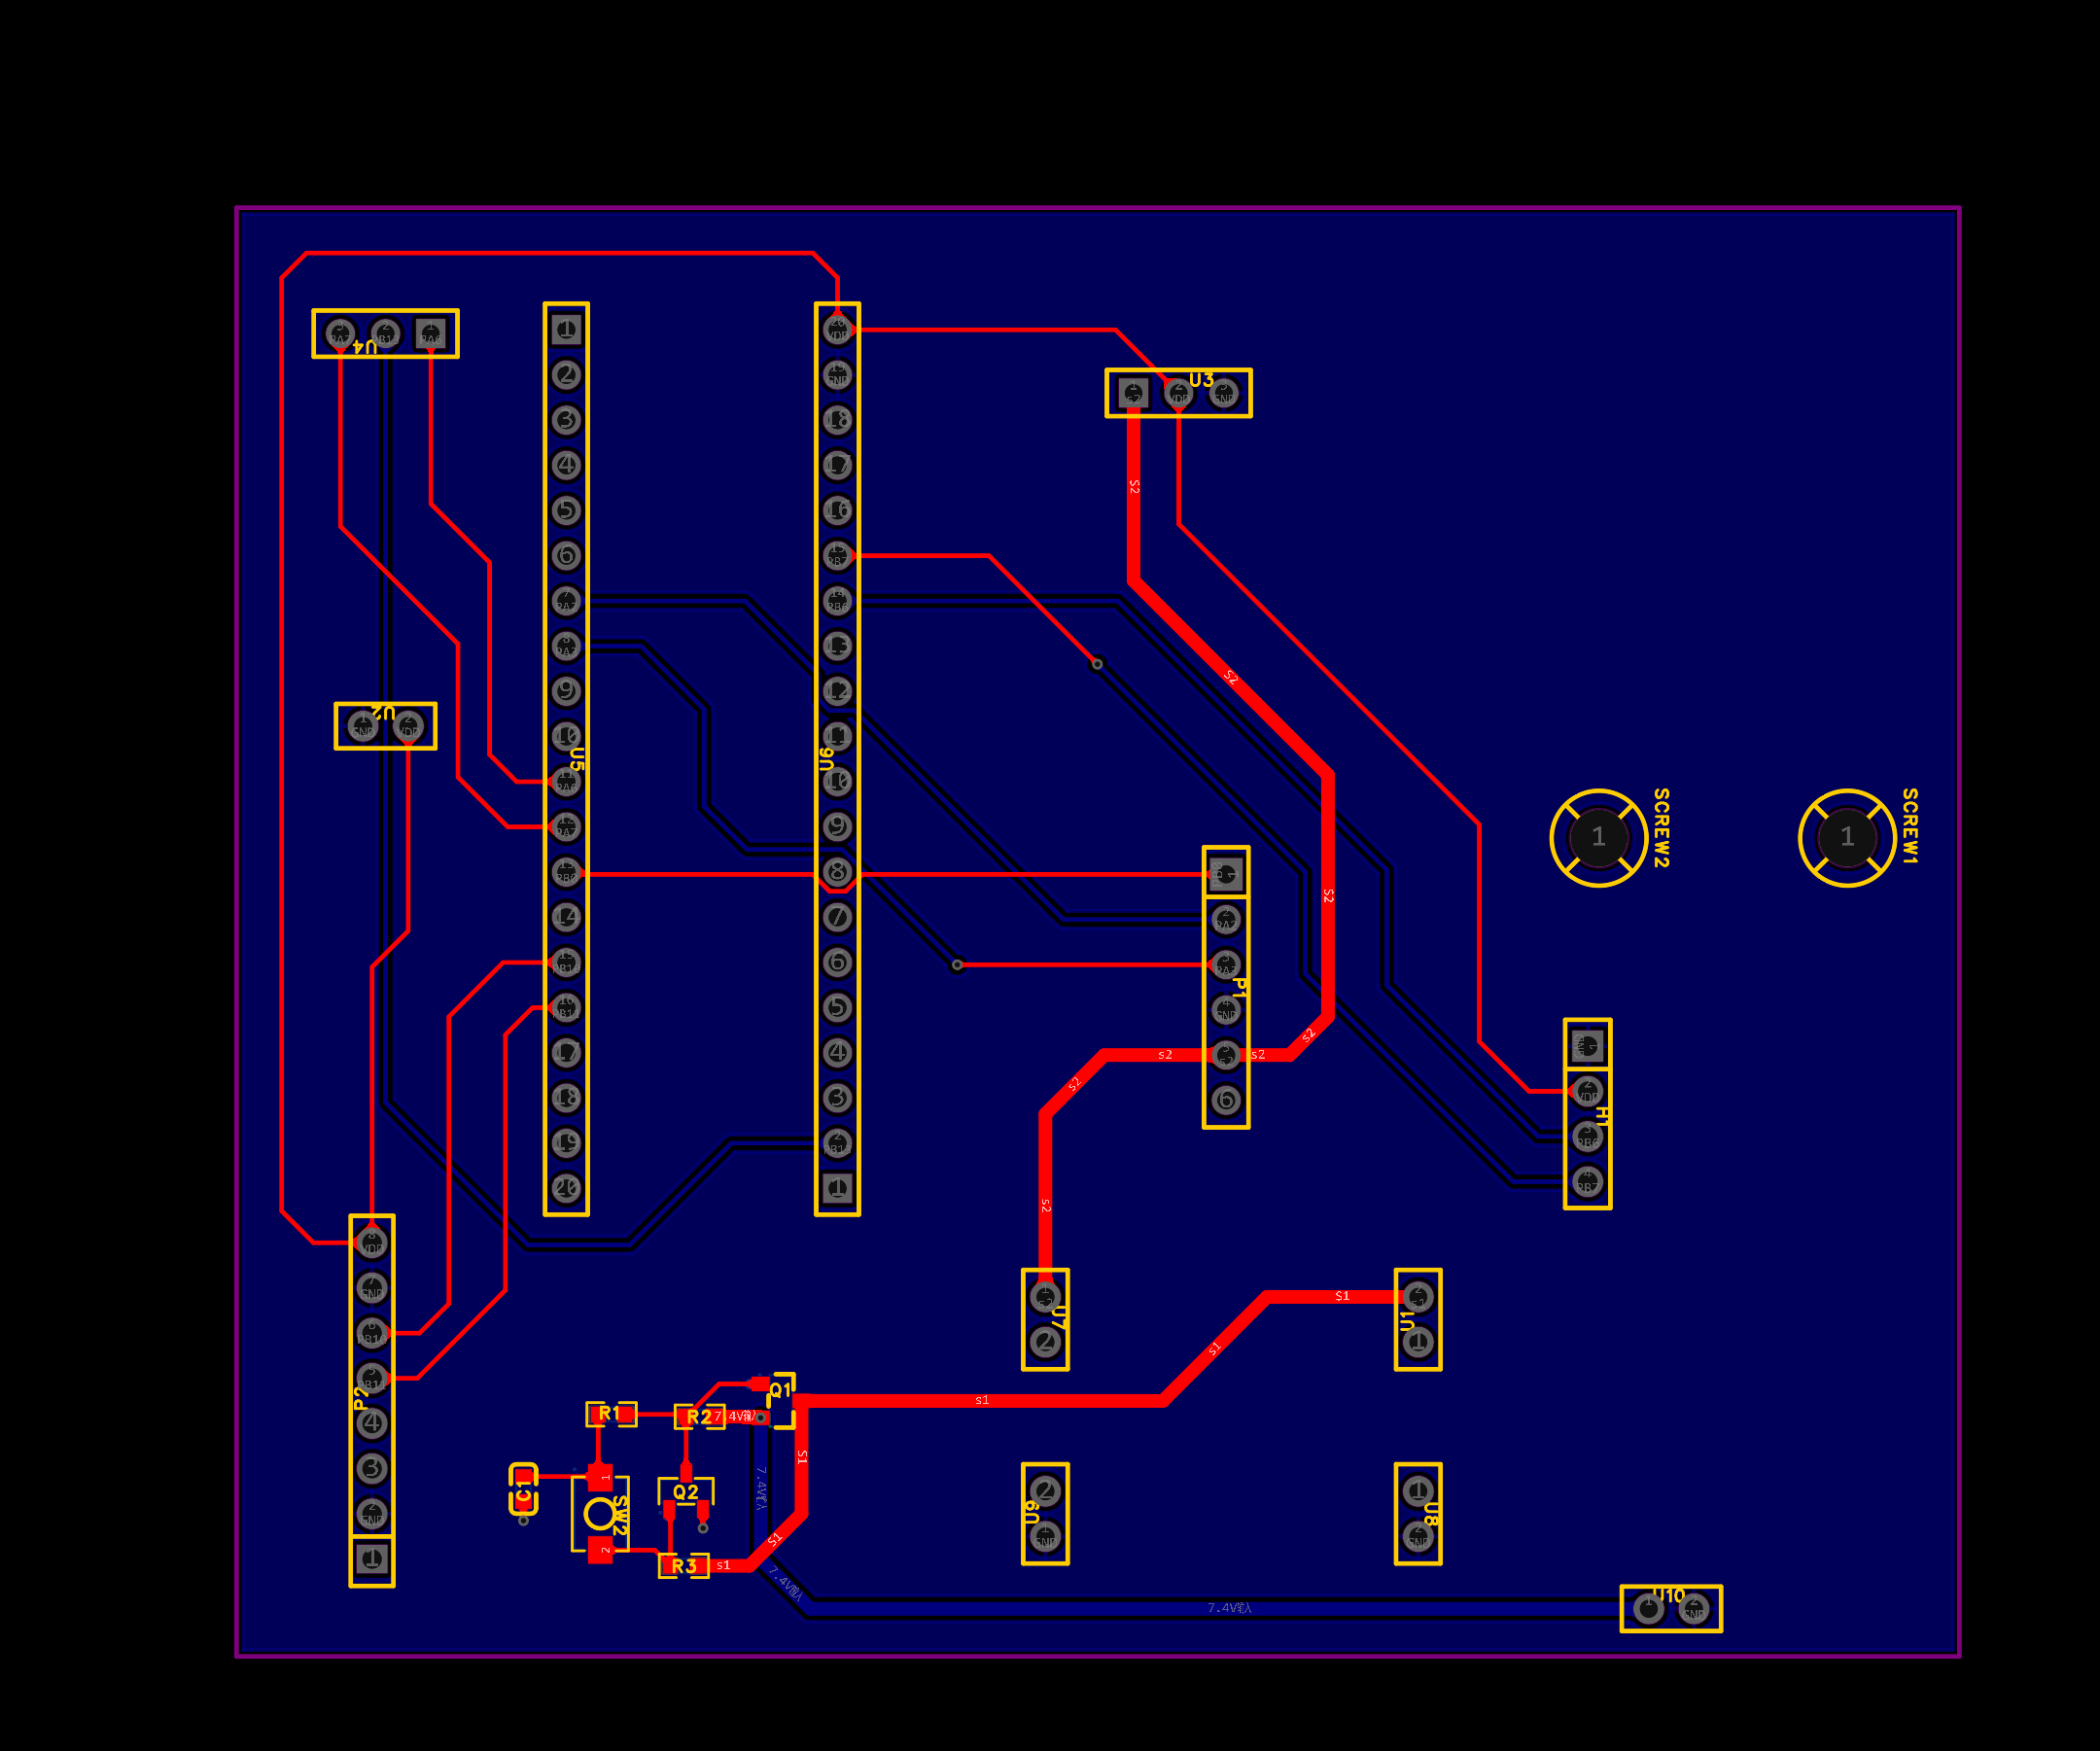
\includegraphics[width=0.95\textwidth]{figures/PCB终版.png}
    \caption{系统PCB板设计图（STM32F103C8T6核心板 + OLED/MPU6050/HC-05布局）}
    \label{fig:full_demo}
\end{figure}

\FloatBarrier